\chapter{Methodology of Chess App}
\label{cha:methodology}

\section*{Introduction of Methodology}

This chapter outlines the methodology employed in the development of \textit{Guardians of the Chess Grandmaster} (GOTCG), an AI-enhanced chess learning platform. The approach combines software development practices with a \textbf{research-informed} methodology to create a comprehensive educational tool for chess players of varying skill levels.

\section{Development Approach}

The project adopted a \textbf{software development methodology} rather than a pure research methodology, prioritizing the creation of a functional, user-centered application that \textbf{leverages} artificial intelligence to enhance chess learning experiences.

\subsection*{Agile and Iterative Development}

An \textbf{agile and incremental approach} was employed throughout the development lifecycle, enabling continuous refinement and adaptation based on testing outcomes and emerging requirements. This methodology \textbf{facilitated} rapid prototyping, continuous integration of user feedback, flexible response to technical challenges, and iterative improvement of core functionalities.

\subsection*{Planning and Requirements Analysis}

Project requirements were determined through market research analyzing existing chess platforms (Chess.com, Lichess), user story development for different skill levels, feature mapping of core functionalities, and technical feasibility studies. Requirements were documented and prioritized using a backlog system, with features categorized by their importance to the minimum viable product (MVP) and subsequent iterations.

\section{Development Process Management}

\subsection*{Version Control and Collaboration}

\textbf{GitHub} was utilized as the primary development tool, providing version control through Git, issue tracking for bug reporting and feature requests, project boards for task management, code review capabilities through pull requests, and documentation hosting. The repository was organized into distinct \texttt{/frontend} and \texttt{/backend} directories.

\subsection*{Development Workflow}

Development followed a structured workflow: feature planning translated \textbf{user stories} into technical tasks; implementation occurred in feature branches with regular commits; testing validated functionality locally; code review ensured quality and \textbf{adherence} to standards; integration merged approved changes; and deployment released updates to production.

\section{Technology Selection and Justification}

\subsection*{Frontend Technologies}

The \texttt{frontend} architecture employed \href{https://18.react.dev/}{\textbf{React 18.3.1}} for its component-based architecture and efficient state management; \href{https://www.typescriptlang.org/docs/handbook/release-notes/typescript-5-6.html}{\textbf{TypeScript 5.6.2}} to enhance code quality through static typing; \textbf{Vite} for fast Hot Module Replacement during development; \href{https://mui.com/material-ui/}{\textbf{Material-UI}} for consistent interface design; and \href{https://motion.dev/docs/react}{\textbf{Framer Motion}} for smooth animations.

\subsection*{Backend Technologies}

The \texttt{backend} infrastructure utilized \textbf{Node.js (v22)} for its non-blocking I/O model essential for concurrent connections; \textbf{Express.js} as the web application framework; \href{https://socket.io/}{\textbf{Socket.IO}} for bidirectional real-time communication; \href{https://firebase.google.com/}{\textbf{Firebase}} for authentication and user profiles; and \href{https://www.mongodb.com/}{\textbf{MongoDB}} for game data storage due to its flexible schema design.

\subsection*{Progressive Web App (PWA) Implementation}

The platform was developed as a PWA to provide cross-device compatibility, offline functionality through service workers, installability without app store distribution, and fast loading times. There are two things for deploying both \texttt{frontend} and \texttt{backend} $\rightarrow$ Vercel and Railway. An example on Figure~\ref{fig:appLogo}
\begin{figure}
    \centering
    
\includegraphics[width=0.35\linewidth]{images//Methodology/icon-192.png}
    \caption{PWA Chess App Logo Design}
    \label{fig:appLogo}
\end{figure}

\section*{Validation and Testing Strategy}

A comprehensive testing strategy was implemented using \textbf{unit testing} to verify individual components; \textbf{integration testing} for API endpoints and database interactions; \textbf{end-to-end testing} for complete user workflows; and \textbf{real-time testing} for WebSocket reliability. Validation included functional testing of all features, performance monitoring, usability evaluation, cross-browser compatibility testing, and responsive design verification across devices.

\section{Research Foundation}

Prior to implementation, research was conducted on chess rating systems (Elo algorithm), chess learning methodologies, existing platform analysis, AI integration in education, and real-time web technologies. This research informed design decisions and feature priorities throughout development. For example on Figure~\ref{fig:rf}

\begin{figure}
    \centering
    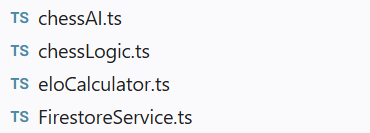
\includegraphics[width=0.45\linewidth]{images//Methodology/Research_Foundation.png}
    \caption{Four files on \texttt{Utils/} has been educated on web technologies}
    \label{fig:rf}
\end{figure}


\section{Problem-Solving Approach}

An \textbf{empirical approach} was employed when addressing technical challenges. Problems were logged and categorized by severity; debugging tools and systematic testing identified root causes; multiple solutions were prototyped and evaluated; selected solutions were implemented and validated; and lessons learned were documented. Key challenges included real-time synchronization across clients, Firebase authentication integration, \textbf{hybrid} database architecture design, PWA configuration, and development environment consistency.

\section{Development Environment and Tools}

The development environment consisted of Node.js v22, npm for package management, Firebase CLI for integration, Git for version control, and Visual Studio Code with relevant extensions. Environment variables were managed through \texttt{.env} files for Firebase configuration, MongoDB connection strings, API endpoints, and service credentials, ensuring sensitive data remained secure while maintaining consistency across environments.

\section{Deployment and Limitations}

The platform was deployed as a Progressive Web App with \texttt{frontend} static file serving, \texttt{backend} API and WebSocket hosting, Firebase authentication services, and MongoDB Atlas for data storage. Limitations included time \textbf{constraints} affecting feature scope, limited access to extensive user testing groups, reliance on third-party services, and single-developer capacity constraints. Here's an example from Figure~\ref{fig:dl}

\begin{figure}
    \centering
    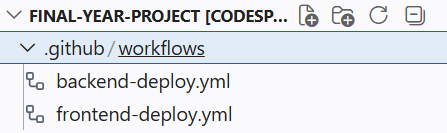
\includegraphics[width=0.45\linewidth]{images//Methodology/Deployment_Limitation.png}
    \caption{Two files of \texttt{.yml} for deploying both to initialised an app}
    \label{fig:dl}
\end{figure}

\section*{Summary}

This methodology chapter has outlined the comprehensive approach taken in developing \textit{Guardians of the Chess Grandmaster}. The agile, iterative development process, combined with careful technology selection and systematic testing, enabled the creation of a functional AI-enhanced chess learning platform. The \textbf{empirical} problem-solving approach and research-informed decision-making ensured that technical challenges were addressed effectively while maintaining focus on user needs and educational objectives.